\documentclass[12pt, a4paper, russian]{article}
\usepackage[margin=2cm]{geometry}
\usepackage[T2A]{fontenc}
\usepackage[utf8]{inputenc}
\usepackage[english,russian]{babel}
\usepackage{amsmath}
\usepackage{subfig}
\usepackage{caption}
\usepackage[compress]{cite}
\usepackage{graphicx}
\usepackage{xcolor}
\usepackage{algorithm}
\usepackage{algpseudocode}
\usepackage{enumitem}
\usepackage{multirow}
\usepackage{booktabs}
\usepackage{titling}
\usepackage[hidelinks]{hyperref}
\usepackage{setspace}
\singlespacing

% To prevent LaTeX from hyphenating
\tolerance=1
\emergencystretch=\maxdimen
\hyphenpenalty=10000
\hbadness=10000

\makeatletter \renewcommand*{\ALG@name}{Алгоритм} \makeatother


%%%%%%%%%%%%%%%%%%%%%%%%%%%%%%%%%%%%%%%%%%%%%%%%%%
\begin{document}

%%%%%%
%%%%%% Информация на английском языке
%%%%%%

\title{Global optimization algorithm that uses decision trees to find local extrema \thanks{The work was supported by the Ministry of Science and Higher Education of the Russian Federation (project no. FSWR-2023-0034), and by the Research and Education Mathematical Center (project no.  075-02-2022-883).}}

\author{D.~I.~Silenko, I.~G.~Lebedev\\
	\small{Lobachevsky State University of Nizhny Novgorod, 603022, Nizhny Novgorod, Russia}
}
\date{}
\maketitle

\begin{small}
\textbf{Abstract:} The paper considers the algorithms for solving the multidimensional global optimization problems using decision tree to reveal the attraction regions of the local minima. We suppose, that the target function is defined as a “black box” and satisfied Lipschitz condition with unknown constant. We propose a method for selecting the local extrema neighborhood of the target function based on analysis of accumulated search information using machine learning methods. This allows us to make a decision to run a local method, which can speed up the convergence of the algorithm. The proposition was confirmed by the results of numerical experiments demonstrating the speedup when solving a series of test problems.

\textbf{Key words:} Global optimization, multiextremal functions, parallel computing, decision tree.
\end{small}

% References
%\renewcommand{\refname}{References}
%\bibliographystyle{IEEEtran}
%\bibliography{articleEng}



%%%%%% 
%%%%%% Информация на русском языке
%%%%%%
\emptythanks
\title{Алгоритм глобальной оптимизации, использующий деревья решений для выявления локальных экстремумов\thanks{Работа выполнена при финансовой поддержке Министерства науки и высшего образования РФ (проект № FSWR-2023-0034) и научно-образовательного математического центра “Математика технологий будущего” (соглашение № 075-02-2022-883).}}

\author{Д. И. Силенко, И. Г. Лебедев\\
	\small{Нижегородский государственный университет им. Н. И. Лобачевского, 603022, Н.Новгород, Россия} 
}
\date{}
\maketitle

УДК 519.853.4

\vspace{\baselineskip}

\begin{small}
\textbf{Аннотация:} В работе рассматривается решение задач многомерной глобальной оптимизации с применением деревьев решений для выявления областей притяжения локальных минимумов. Предполагается, что целевая функция задачи задана как «черный ящик» и удовлетворяет условию Липшица с априори неизвестной константой. Мы предлагаем способ выделения окрестностей локальных экстремумов целевой функции на основе анализа накопленной поисковой информации средствами машинного обучения. Это позволяет принять решение о запуске локального метода для уточнения значения функции в локальном минимуме, что может ускорить сходимость алгоритма. Выдвинутое предположение подтверждается результатами вычислительных экспериментов, демонстрирующих ускорение при решении серии тестовых задач.

\textbf{Ключевые слова:} деревья решений, глобальная оптимизация, многоэкстремальные функции, локальная оптимизация.
\end{small}


\section{Введение}

В прикладных задачах нередко возникает необходимость использования глобальной оптимизации. При этом необходимо уменьшить число проводимых в ходе работы алгоритма операций, так как любое вычисление значения функции - трудоемкая задача. Это накладывает дополнительные требование на то, какой подход к решению задачи выбрать. Самих подходов достаточно много, и они реализуют разные идеи: от случайного поиска \cite{fio_bib1, fio_bib2, fio_bib3}, до детерминированного \cite{fio_bib4, fio_bib5, fio_bib6}. Однако, учитывая все требования, для наших целей нам лучше всего подходит алгоритм глобального поиска (AGS). В процессе поиска он рассматривает не все варианты, а отбирает лучшие по некоторым критериям. В статье мы попробуем объединить АГП и метод локальной оптимизации (метод Хука-Дживса), применяя деревья решений. В теории, они должны дополнительно уменьшить количество проводимых итераций. А это приведет к непосредственному уменьшению вычислений целевой функции в общем.

Методы локальной оптимизации используются для решения более простых задач: когда необходимо найти один из локальных экстремумов функции (точки, в которой целевая функции принимает минимальное или максимальное значение) в области ее определения.

Для того, чтобы понять, в какой момент лучше всего запускать локальный метод, мы используем алгоритм на основе деревьев решений. Мы накапливаем определенное число точек и лишь когда их станет достаточно начинаем обработку. Эти полученные точки мы используем для тренировки деревьев решений и предсказания по нему. Предсказание позволяет нам получить кусочно-линейную аппроксимацию по этому дереву. После чего мы рассматриваем уже полученную по дереву аппроксимацию. Проверяем значения соседних точек к той, которую считаем подозрительной на минимум, и оцениваем попали мы в область притяжения локального минимума или нет. 

\section{Постановка задачи}

Рассмотрим задачу глобальной оптимизации с целевой функцией $\varphi(y)$ на гиперинтервале $D=\{ y\in\ R^N:\ a_i\le\ y_i\le\ b_i,\ 1 \le\, i\le\ n \}$. Для решения задачи, необходимо выдвинуть дополнительное требование к виду функции - предположим, что она удовлетворяет условию Липшица. Значение этой константы нам заранее неизвестно $L$. Условие Липшица дает нам  ограниченные вариации значений функций при ограниченных изменениях её аргументов. При решение прикладных задач, это предположение можно интерпретировать как указание на ограниченную способность моделируемой системы к изменениям. 



%%%%%%%%%%%%%%%%%%%%%
\begin{equation} \label{sec:problem}   
	\varphi(y^*) = min\{\varphi(y):y\in D\}, D = \{y \in R^N : a_i \leq y_i \leq b_i, 1 \leq i \leq N \},
\end{equation}
где $a,b \in R$ --- заданные векторы.


\begin{displaymath}
	|\varphi(y_1)-\varphi(y_2)|\leq L\parallel y_1-y_2 \parallel
	,y_1,y_2 \in D, 0<L< \infty.
\end{displaymath}




При численном решении задачи (\ref{sec:problem}) возможно построить лишь оценку $y_k^\ast\in D$ на основе числа проведенных итераций $k$. Чтобы такую оценку можно было использовать как решение задачи, она должна соответствовать выбранному критерию близости к реальной оптимальной точке $y^\ast$. В качестве примера можно рассмотреть следующий критерий: ${ ||y^\ast -y}_k^\ast||\le\ \varepsilon$, где $\varepsilon\geq0$ — заданная точность. Отдельно отметим оптимизируемую функцию $\varphi(y)$. Она не обязана быть представлена в аналитическом виде. Это может быть результат работы подпрограммы или библиотеки, что расширяет область ее возможного применения.

Итак, мы решаем многоэкстремальные многомерные задачи глобальной оптимизации. Стоит отметить, что каждый термин в данном описании накладывает свои трудности. Задачи многоэкстремальной оптимизации выделяются на фоне других задач оптимизации в силу более высокой сложности решения. Глобальная оптимальность требует проведения поиска на всей заданной области, сузить ее заранее невозможно. А многомерность ведет к тому, что при росте размерности, трудоемкость поиска решения растет экспоненциально. В итоге, необходимо построить покрытие в области параметров (так называемая сетка) и выбирать в этой области оптимальное значение функции. 


\section{Многомерный алгоритм глобального поиска}

Алгоритм глобального поиска основан на идее, что минимизируемая функция представляет из себя случайный процесс. При выполнении каждой новой итерации, найденная точка сохраняется в списке известных значений и  процесс повторяется. Главное в подобных алгоритмах --- решающее правило и оно в АГП сконструировано таким образом, чтобы каждая последующая итерация проводилась в глобальном минимуме математического ожидания значения функции. Более подробно работа алгоритма будет представлена ниже. Критерий остановки --- это правило, согласно которому алгоритм определяет, необходимо завершить работу или продолжить выполнение. В качестве такого правила может быть выбран один из следующих подходов: 
\begin{enumerate}
	\item Достигнут заданный максимум по числу возможных итераций. 
 \item Новая точка не будут получена рядом с истинным глобальным минимумом.
	\item Расстояние между двумя точками не будет меньше заданного значения.
\end{enumerate}

При решении многомерных задач применяется редукция размерности (т.е. сведение многомерной задачи к эквивалентной одномерной) с использованием кривых Пеано. Это позволяет не рассматривать задачу на всей области поиска $D$, а ограничиться лишь минимизацией на отрезке $[0, 1]$

\begin{equation*}
	\phi({y(x}^\ast))\ =\ min\{\phi(y(x)):\ x\in[0,\ 1]\}.
\end{equation*}
Условие Липшица, выдвинутое нами при постановке задачи, при таком переходе в первозданном виде применить нельзя. Однако оно может быть преобразовано в эквивалентное равномерное условие Гельдера
\begin{equation*}
	\left|\phi (y \left(x_1\right))- \phi (y \left(x_2\right)\right )|\le\ H\left|x_1-x_2\right|^\frac{1}{N},\ x_1,\ x_2\in[0,1]		
\end{equation*}

Проделанные таким образом преобразования позволяют рассматривать минимизацию одномерной функции $f(x)\ =\ \phi(y(x)), \ x\in [0,1]$. Общность рассуждений при этом нарушена не будет. 

Схема алгоритма:

На подготовительном шаге параллельно проводятся $p$ поисковых испытаний в произвольных внутренних точках $x^1, ...,x^p$ отрезка $[0,1]$, что соответствует первой итерации  алгоритма. 

Если выполнено $n\geq1$ итераций, которым соответствуют $k=k(n)$ проведенных поисковых испытаний в точках $x^i, 1\leq i\leq k$, то точки $x^{k+1},\ldots,x^{k+p}$ испытаний следующей $(n+1)$-й итерации будут определять следующим образом.

\begin{enumerate}

	\item  Перенумеровать (нижним индексом) точки ранее проведенных испытаний $x^i, 1\leq i\leq k$, а также граничные точки отрезка [0,1] в порядке возрастания координаты:
 \begin{displaymath}
		\label{agp1_sort}
	0=x_0<\ x_1<\ ...\ <x_{k+1}=1.
	\end{displaymath}
	и сопоставить им значения $z_i=f(x_i)$. 
	
	\item  Вычислить текущие нижние оценки $M$ неизвестной константы Гельдера $H$:
 \begin{displaymath}
		\label{agp2_mu}
	\mu=max\left\{\frac{|z_i-z_{i-1}|}{{{(x}_i-x_{i-1})}^{1/N}},\ i=1,\ldots,k\right\},\ M=\ \left\{\begin{matrix}r\mu,\ \mu>0,\\1,\ \mu=0,\\\end{matrix}\right.\
	\end{displaymath}
	где $r>1$ --- параметр алгоритма.
   
	\item  Для всех интервала $(x_{i-1},x_i), 1\leq i\leq k+1,$ вычислить значение $R(i)$, называемое \textit{характеристикой} интервала, в соответствии с формулами
	\begin{displaymath}
		\label{agp3_R1}
		R(1)=2\Delta_1-4\dfrac{z_1}{M}, \; R(k+1)=2\Delta_{k+1}-4\dfrac{z_k}{M},
	\end{displaymath}
	\begin{displaymath}
		\label{agp3_Ri}
		R(i)=\Delta_i+\dfrac{(z_i-z_{i-1})^2}{M^2\Delta_i}-2\dfrac{z_i+z_{i-1}}{M},1<i<k+1,
	\end{displaymath}
	где \(\Delta_i=(x_i-x_{i-1})^\frac{1}{N}\).
   
	\item   Упорядочить характеристики $R\left(i\right),\ 1\leq i \leq k+1,$ в порядке невозрастания 
	
	%%%%%%%%%%%%%%%%%%%%%
	\begin{equation}
		\label{agp4_R_sort}
	R\left(t_1\right)\geq\ R\left(t_2\right)\geq...\geq\ R\left(t_k\right)\geq\ R(t_{k+1}),\ 
	\end{equation}	
	и выбрать интервал с номерами $t$, с наибольшими значениями характеристики.

	\item  В выбранном интервале вычислить точку $x^{k+1}$, в соответствии с формулами
	\begin{displaymath}
		\label{agp5_x1}
	x^{k+j}=\frac{x_{t_j}+x_{t_j-1}}{2},\ t_j=1,\ t_j=k+1,
	\end{displaymath}	
	\begin{displaymath}
		\label{agp4_xi}	
	x^{k+1}=\frac{x_{t_j}+x_{t_j-1}}{2}-sign\left(z_{t_j}-z_{t_j-1}\right)\frac{1}{2r}\left[\frac{\left|z_{t_j}-z_{t_j-1}\right|}{\mu}\right]^N,\ 1<t_j<k+1.
	\end{displaymath}	

\end{enumerate}

Отметим, что в прикладных оптимизационных задачах процесс проведения испытания является, как правило, значительно более трудоемким по сравнению с работой вычислительных правил алгоритма.

Алгоритм останавливает свою работу в случае, если значения $t$ из (\ref{agp4_R_sort}) выполняется условие \(\Delta_{t_j} < \varepsilon\). Данный критерий остановки (наряду с обычным для итерационных методов критерием, ограничивающим число выполненных итераций) используется в задачах оптимизации, в которых точка глобального минимума $x^*$ заранее неизвестна. 
	 
При решении тестовых задач, в которых точка глобального минимума $x^*$ является  известной, можно использовать также и критерий остановки по попаданию в окрестность глобального минимума. В этом случае алгоритм останавливает свою работу, если хотя бы для одного $t_j,\ 1\le\ j\le\ p$ из (\ref{agp4_R_sort}) выполняется условие $\left|x_{t_j}-\ x^\ast\right| < \varepsilon.$
	
Результатом работы АГП при решении рассматриваемой задачи, является оценка глобального оптимума:
\begin{displaymath}
	f_k^*=\min_{1\leq i \leq k}f(x_i), \; x_k^*=arg \min_{1\leq i \leq k}f(x_i).
\end{displaymath}



В \cite{fio_bib20} приведено обоснование данного способа организации вычислений. А в работе  \cite{fio_bib11} представлены модификации, учитывающие наличие ограничений-неравенств, а также информацию о значение производной целевой функции, 

\section{Метод Хука-Дживса}

 Метод Хука-Дживса был выбран нами как достаточно эффективный и простой в реализации алгоритм локальной оптимизации. Он состоит из двух частей.  \cite{fio_bib14, fio_bib15}. Первая часть - исследующий поиск - включает в себя несколько шагов:
 \begin{enumerate}
 	\item	Определяется значение шага (может меняться в процессе поиска и различно для каждой координаты).

 	\item	Сделать шаг по текущей координате. Шаг поиска будет успешным, если значения целевой функции в контрольных точках не превышают исходных значений целевой функции.

 	\item	В противном случае нужно вернуться к предыдущему пункту и сделать шаг в обратном направлении. 

 	\item	После того как будут пройдены все $N$ параметров, исследующий поиск заканчивается. Найденная точка называется базовой.
 \end{enumerate}

 Вторая часть - поиск по образцу - состоит из выполнения одного шага от полученной базовой точки вдоль линии, соединяющей ее с предыдущей базовой точкой. Величина этого шага определяется задаваемым заранее параметром.

 На рисунке (\ref{fig:fig1}) приведен небольшой пример работы алгоритма. Отображены линии уровней функции, закрашенными  кружками обозначены успешные шаги, не закрашенные --- неуспешные шаги при исследующем поиске.

 \begin{figure}[!h]
	\begin{center}
		\begin{minipage}[h]{0.8\linewidth}
			
\includegraphics[width=1\linewidth]{figure/fig1.pdf}
			\caption{Пример итераций алгоритма Хука-Дживса} %% подпись к рисунку
			\label{fig:fig1}
		\end{minipage}
	\end{center}
 \end{figure}	

\section{Деревья решений}

Деревья решений --- это метод автоматического анализа больших массивов данных, который применяется в машинном обучении. Дерево решений представляет собой бинарное дерево (дерево, в котором каждый не листовой узел имеет два дочерних узла). Такая структура позволяет использовать подобное дерево в машинном обучении (причем как для решения задач классификации, так и для регрессионных задач) в целях автоматизации анализа большого объема данных. Для задач регрессии, каждому листу дерева присваивается константа, как следствие  получаемая функция аппроксимации является кусочно-постоянной. А вот для классификации подход иной: каждый лист дерева помечается меткой класса, при этом несколько листьев могут иметь одну и ту же метку. 

Процедура прогнозирования по дереву решения начинается с корня. От каждого не листового узла процедура идет вправо или влево в соответствии со значением переменной (ее индекс хранится в наблюдаемом узле). 

Возможны следующие переменные:
\begin{enumerate}

	\item Категориальные переменные --- значение дискретной переменной проверяется на предмет того, принадлежит ли оно определенному подмножеству значений (также хранящемуся в узле) из набора допустимых величин. Если принадлежит, то идем влево. В противном случае --- вправо. 

	\item Упорядоченные переменные --- значения которых сравнивается с порогом (который также хранится в узле). Если значение больше порога, процедура идет вправо. В противном случае --- влево.
\end{enumerate}

Как только алгоритм достигает конечного узла, в качестве ответа процедуры прогнозирования выбирается значение, присвоенное этому узлу. 

В нашем случае дерево решений строит функцию $\varphi(y)$ кусочно постоянную аппроксимацию $\varphi(y)$  в многомерном пространстве, обозначим как $z' = \psi(y)$ значение вычисленное по дереву решения в точке $y$.

Библиотека алгоритмов компьютерного зрения, обработки изображений и численных алгоритмов общего назначения с открытым кодом OpenCV \cite{Brahmbhatt2013} предоставляет уже готовые к использованию деревья решений. В данной работе, при разработке алгоритма, применяющего деревья решений для выявления областей притяжения локальных минимумов, мы использовали данную библиотеку. И, следовательно, все подробности внутренней реализации деревьев решений можно найти в соответствующей документации - \cite{fio_bib16}

\begin{figure}[ht!]
	\begin{center}
			\begin{minipage}[h]{0.8\linewidth}
					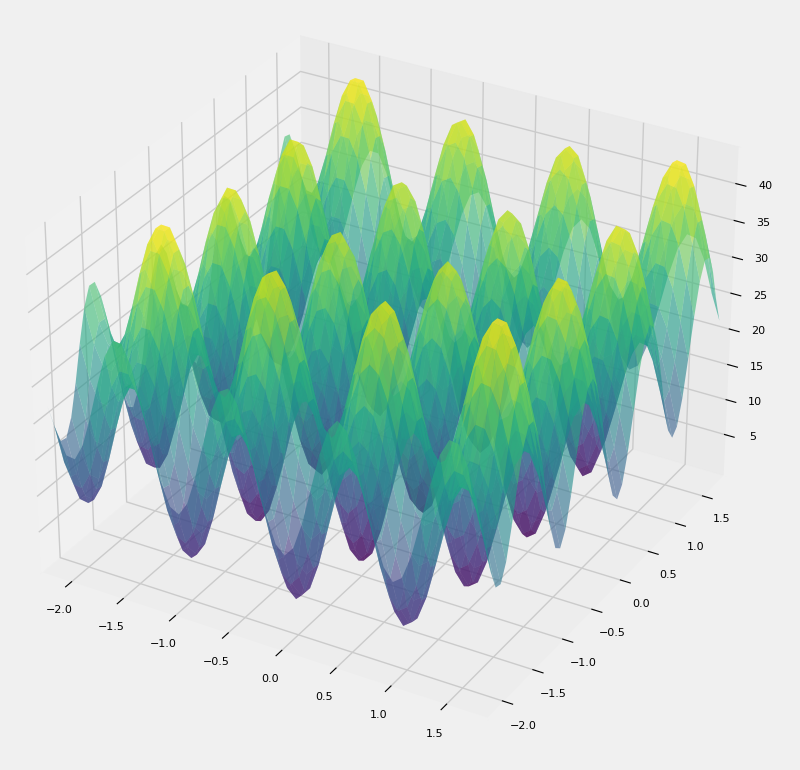
\includegraphics[width=1\linewidth]{figure/Figure_1}
					\caption{Функция Растригина} %% подпись к рисунку
					\label{fig:fig2}
				\end{minipage}
		\end{center}
\end{figure}	

\begin{figure}[ht!]
	\begin{center}
			\begin{minipage}[h]{0.8\linewidth}
					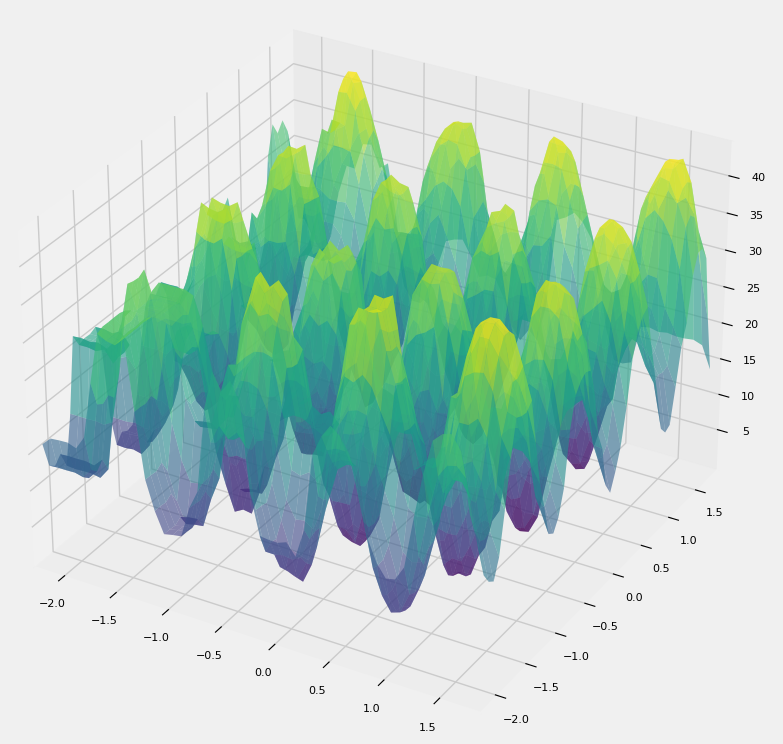
\includegraphics[width=1\linewidth]{figure/Figure_2}
					\caption{Аппроксимация по двумерному дереву решений} %% подпись к рисунку
					\label{fig:fig2_2}
				\end{minipage}
		\end{center}
\end{figure}	

На рисунке  (\ref{fig:fig2}) отображена трехмерная поверхность  оптимизационной задачи (Функции Расстрига), и на рисунке  (\ref{fig:fig2_2}) отображена аппроксимация   построенная по дереву решений. 

\section{Объединение локального метода и АГП в случае многомерных задач}

В текущем разделе приведем подробное описание того, как использовать деревьев решений в многомерном случае. В процессе работы АГП необходимо определить, стоит ли использовать текущую точку, в качестве стартовой для локального метода или нет. Для этого можно осмотреть соседние точки испытания. Если среди них есть хоть одна, значение функции в которой больше, чем в текущей, то продолжать работу бессмысленно. В противном случае, можно предположить, что мы находимся в области притяжения локального минимума и можно запустить локальный метод, чтобы быстрее сойтись к минимуму. Использование проекций многомерных точек на одномерный отрезок после редукции размерности (то, что позволяют сделать кривые Пеано) нам для этих целей не подойдут по нескольким причинам. Во-первых, функция после отображения сильно изменяется, один локальный минимум в многомерном пространстве может разделиться на множество минимумов после отображения. Во-вторых, после отображения информацию о взаимном расположении точек исходной функции может быть искажена. Точки, расположенные близко в многомерном пространстве, могут оказаться на разных концах одномерного отрезка и наоборот).




Поэтому мы будем работать именно с исходными точками. Однако определить соседние точки в многомерном пространстве достаточно трудоемко, и для этого мы будем использовать деревья решений. 

После проведения определенного числа испытаний (например, $100\ \ast\ N$), используем все накопившиеся точки для инициализации подходящей структуры данных и тренировки на ее основе дерева решений. Чтобы проще было определить соседние точки, мы построим равномерную сетку с определенным шагом по каждой из размерностей, после чего передадим эти точки на вход предсказанию по дереву. Теперь, имея равномерную сетку точек и зная значение функции в каждой из них, найдем ближайшую, с точки зрения евклидова расстояния, к исходной. Эта ближайшая точка является проекцией изначальной точки на равномерную сетку и что бы определить  ее соседей, достаточно  просто перебрать индексы соседей. К тому же поскольку дерево решений строит аппроксимацию исходной задачи (пусть и кусочно постоянную) мы можем оценить значение функции в тех областях, в которых испытания ранее не проводились.

При рассмотрении соседей необходимо учитывать следующее: если хоть один из соседей имеет значение функции меньшее, чем в текущей точке, то запуск локального метода не нужен; если какой-то из соседей имеет значение функции такое же, как в текущей, то его также необходимо проверить (найти всех его соседей и проверять их аналогично); и только в том случае, если все значения функций соседей больше (включая соседей равных точек) мы можем запускать локальный метод. Ниже представлен алгоритм глобального поиска, учитывающий описанные ранее модификации:


\begin{enumerate}
	
	\item  Перенумеровать (нижним индексом) точки ранее проведенных испытаний $x^i, 1\leq i\leq k$, а также граничные точки отрезка [0,1] в порядке возрастания координаты:
	\begin{displaymath}	
	0=x_0<\ x_1<\ ...\ <x_{k+1}=1.
	\end{displaymath}
	и сопоставить им значения $z_i=f(x_i)$. 

	\item  Вычислить текущие нижние оценки $M$ неизвестной константы Гельдера $H$:
	\begin{displaymath}	
	\mu=max\left\{\frac{|z_i-z_{i-1}|}{{{(x}_i-x_{i-1})}^{1/N}},\ i=1,\ldots,k\right\},\ M=\ \left\{\begin{matrix}r\mu,\ \mu>0,\\1,\ \mu=0,\\\end{matrix}\right.\
	\end{displaymath}
	где $r>1$ --- параметр алгоритма.

	\item  Для всех интервала $(x_{i-1},x_i), 1\leq i\leq k+1,$ вычислить значение $R(i)$, называемое \textit{характеристикой} интервала, в соответствии с формулами
	\begin{displaymath}
	R(1)=2\Delta_1-4\dfrac{z_1}{M}, \; R(k+1)=2\Delta_{k+1}-4\dfrac{z_k}{M},
	\end{displaymath}
	\begin{displaymath}
	R(i)=\Delta_i+\dfrac{(z_i-z_{i-1})^2}{M^2\Delta_i}-2\dfrac{z_i+z_{i-1}}{M},1<i<k+1,
	\end{displaymath}
	где \(\Delta_i=(x_i-x_{i-1})^\frac{1}{N}\).

	\item   Упорядочить характеристики $R\left(i\right),\ 1\leq i \leq k+1,$ в порядке невозрастания 
	\begin{displaymath}
	R\left(t_1\right)\geq\ R\left(t_2\right)\geq...\geq\ R\left(t_k\right)\geq\ R(t_{k+1}),\ 
	\end{displaymath}	
	и выбрать интервал с номерами $t$, с наибольшими значениями характеристики.

	\item  В выбранном интервале вычислить точку $x^{k+1}$, в соответствии с формулами
	\begin{displaymath}
	x^{k+j}=\frac{x_{t_j}+x_{t_j-1}}{2},\ t_j=1,\ t_j=k+1,
	\end{displaymath}	
	\begin{displaymath}
	x^{k+1}=\frac{x_{t_j}+x_{t_j-1}}{2}-sign\left(z_{t_j}-z_{t_j-1}\right)\frac{1}{2r}\left[\frac{\left|z_{t_j}-z_{t_j-1}\right|}{\mu}\right]^N,\ 1<t_j<k+1.
	\end{displaymath}	


	\item  Получить вычисленное  значение функции с процесса $j$, добавить новый trial $z_j = f(y(x_j))$, к множеству $V$. 

	%X_k=\left\{x^1,x^2,\ldots,x^{k+p}\right\}


	\item 	Если $ k\ <\ 100\ast\ N$, то вернуться к шагу 1.

	%\item 	Если используем decision tree не впервые, то перейти к пункту 15.

	\item Создаем дерево решений по множеству $I_k$, получаем функцию аппроксимации  $\psi(y)$.



	\item 	Если используем дерево решений впервые, то строим равномерную сетку

	\begin{displaymath}
	Y'=\{ y'\in\ R^N:\ a_i\le\  {y'_i}^k \le\ b_i,\ 1\le\ i\le\ N,\ 1\le k\le\ \sqrt[N]{300}  \}
	\end{displaymath}

	\item 	Вычисляем значения аппроксимации: $Z' = \{ z'=  \psi(y'), y' \in Y'\}$

	\item Для всех точек $y'\in V$:

	Находим точку $y'_q$ ближайшую  к $y'$,

	Производим обход соседей $y'_q$ по описанному ранее принципу.

	Если ни у одной соседней точки не нашлось значений функции меньших, чем в $y'_q$, то запускаем локальный метод.

	Очищаем множество $V$.


\end{enumerate}




Все полученные результаты были добавлены в систему globalizer \cite{fio_bib18}.
Если говорить более конкретно, то была внедрена система  построения дерева решений, равномерной сетки и прочих сопутствующих вычислений. Использовалась данная система при реализации схемы с запуском локальных методов в нужный момент.  
Ниже приведена блок-схема того, как данная схема была объединена с АГП (\ref{fig:fig3}).

\begin{figure}[ht!]

	\begin{center}
		\begin{minipage}[h]{0.9\linewidth}
			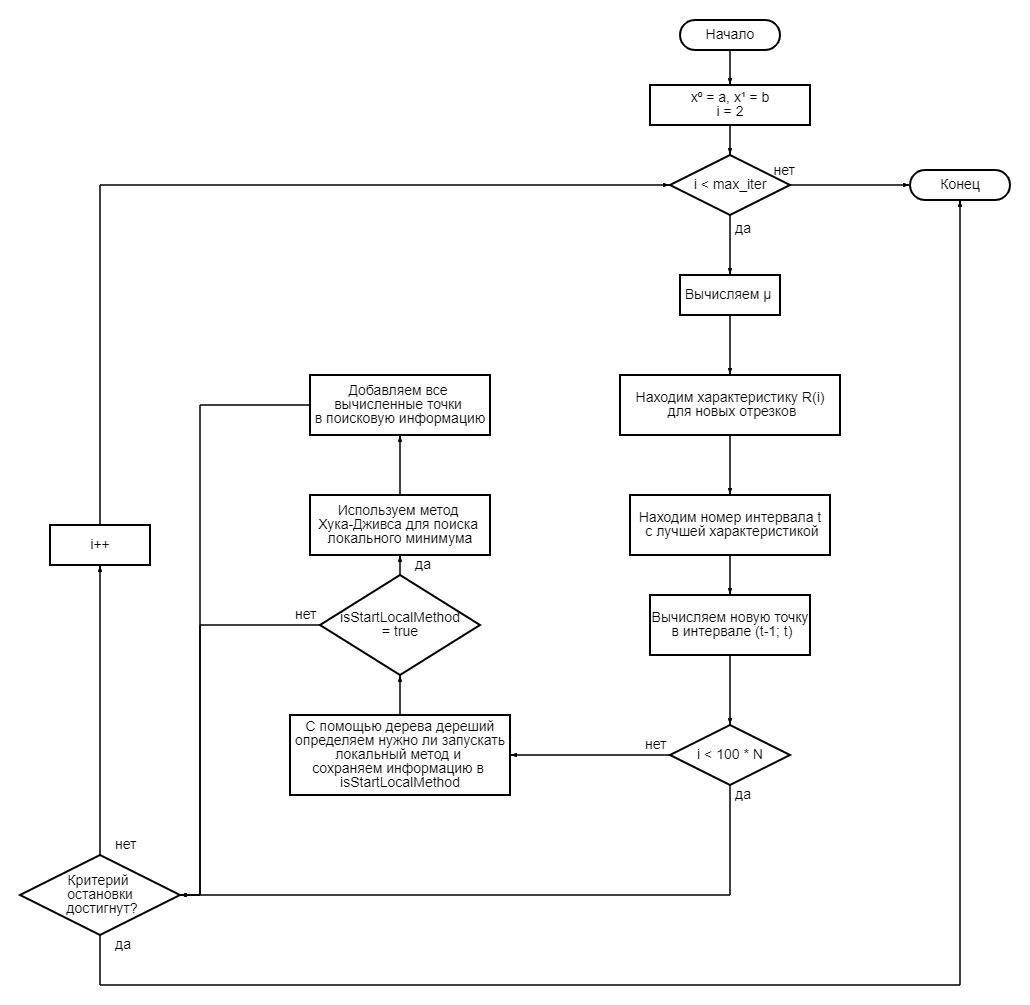
\includegraphics[width=1\linewidth]{figure/fig3.png}
			\caption{Блок-схема объединения АГП и метода Хука-Дживса с использованием дерева решений} %% подпись к рисунку
			\label{fig:fig3}
		\end{minipage}
	\end{center}
\end{figure}	

\section{Эксперименты}

Вычислительные эксперименты были проведены на компьютере со следующими характеристиками: операционная система Windows 11, процессор: Intel(R) Core™ i5-8250U CPU @ 1.60 GHz, 12 Gb RAM.

Работы \cite{fio_bib13, fio_bib17} описывают генераторы GKLS, которые могут генерировать многоэкстремальные задачи оптимизации с известными свойствами: глобальным минимумом и его значением, количеством локальных минимумов и так далее.

В таблице \ref{tab:1} приведено среднее количество итераций методов глобальной оптимизации при решении серии задач из генератора GKLS. Знак «>» указывает на ситуацию, когда не все задачи были решены, в скобках указано количество нерешенных задач. Как видно, АГП превосходит методы DIRECT и DIRECTl по среднему числу итераций. 


\begin{table}[!ht]
    \caption{Среднее число итераций}
    \label{tab:1}
    \centering
    \begin{tabular}{|l|l|l|l|l|}
    \hline
        N & Problem class & DIRECT & DIRECTl & АГП  \\ \hline
        4 & Simple & >47282 (4) & 18983 & 11953  \\ \hline
        ~ & Hard & >95708 (7) & 68754 & 25263  \\ \hline
        5 & Simple & >16057 (1) & 16758 & 15920  \\ \hline
        ~ & Hard & >217215 (16) & >269064 (4) & >148342 (4)  \\ \hline
    \end{tabular}
\end{table}

В таблице \ref{tab:2} приведены результаты сравнения двух алгоритмов –-- многомерного алгоритма глобального поиска (АГП) и АГП с использованием деревьев решений для выявления областей притяжения локальных минимумов (Деревья решений). Численное сравнение проводилось на классах функций Simple и Hard размерности 2, 3, 4 и 5 из \cite{fio_bib19}. Алгоритм прекращал свою работу как только поражалась точка испытания в эпсилон окрестность истинного глобального минимума. 

\begin{table}[h!]
    \caption{Среднее число итераций и среднее число испытаний, проводимое разными алгоритмами}
    \label{tab:2}
    \centering
    \begin{tabular}{|c|c|c|c|c|c|}
    \hline
	
        N & Класс задачи & \multicolumn{2}{c|}{Среднее число итераций} & \multicolumn{2}{c|}{Среднее число точек испытаний} \\ \hline
          & ~ & АГП & Деревья решений & АГП & Деревья решений \\ \hline
          & Simple & 2350.0 & 247.4 & 2348.0 & 390.0  \\ \hline
        2  & Hard & 4732.3 & 353.6 & 4730.3 & 1101.1  \\ \hline
          & Simple & 2115.5 & 579.5 & 2113.5 & 2441.4  \\ \hline
        3  & Hard & 5347.4 & 588.1 & 5345.4 & 2532.7  \\ \hline
          & Simple & 12168.9 & 768.2 & 12166.9 & 3582.2  \\ \hline
        4  & Hard & 25636.5 & 960.0 & 52634.5 & 5171.6  \\ \hline
          & Simple & 20633.5 & 978.0 & 20631.5 & 4840.4  \\ \hline
        5  & Hard & 161094.9 (4) & 1217.0 & 161092.9 (4) & 7115.5  \\ \hline
    \end{tabular}
\end{table}

Среднее число точек испытаний, практически везде, уменьшилось, хотя эти значения и могут быть выше, чем среднее число испытаний (ускорение по которым достаточно велико, вне зависимости от сложности задачи и ее размерности). Объясняется это тем, что в точках испытаний учитываются и те значения, которые в процессе своей работы ставил локальный метод, а их может быть довольно много.


\section{Заключение}



В результате работы нами были успешно совмещены алгоритм глобального поиска с локальным поиском минимума (метод Хука-Джевса). Теоретические свойства рассматриваемого алгоритма удалось подтвердить на практике: серии из сотни тестовых задач показали ускорение по числу проводимых итераций.

%
% ---- Bibliography ----
%
\renewcommand{\refname}{Список литературы}
\bibliographystyle{IEEEtran}   %%link to spmpsci.bst
\bibliography{article}        %%link to article.bib


\section*{Сведения об авторах}

\paragraph{Лебедев Илья Генадьевич} --- заведующий лабораторией суперкомпьютерных технологий и высокопроизводительных вычислений кафедры математического обеспечения и суперкомпьютерных технологий института информационных технологий, математики и механики, Нижегородский государственный университет им. Н.И. Лобачевского  e-mail: \url{ilya.lebedev@itmm.unn.ru}. Область профессиональных интересов: методы глобальной и локальной оптимизации, параллельные алгоритмы, программирование для графических процессоров, CUDA. Является автором и соавтором более 30 научных работ в указанных областях.

\paragraph{Дмитрий Игоревич Силенко} --- окончил бакалавриат института информационных технологий, математики и механики Нижегородского государственного университета им. Н. И. Лобачевского в 2021 году. В настоящее время является магистрантом института информационных технологий, математики и механики (направление - прикладная математика и информатика). Область научных интересов включает методы глобальной и локальной оптимизации, а также технологии параллельных вычислений и параллельные алгоритмы. e-mail: \url{silenko@itmm.unn.ru}. Является соавтором нескольких научных работ в указанных областях.



\paragraph{Контактный номер телефона:}{+7(910)898-02-39}

\section*{Authors' bio}

\paragraph{Ilya~G.~Lebedev} --- Head of the Laboratory of Supercomputer Technologies and High-Performance Computing, Department of Mathematical Software and Supercomputing Technologies, Institute of Information Technology, Mathematics and Mechanics, Nizhny Novgorod State University. N.I. Lobachevsky. e-mail: \url{ilya.lebedev@itmm.unn.ru}. His research interests include algorithms of global and local optimization, parallel algorithms, GPU programming, CUDA. He is the author or coauthor more than 30 papers in these areas.



\paragraph{D. I. Silenko} --- Graduated the Institute of Information Technology, Mathematics and Mechanics of the Lobachevsky State University of Nizhni Novgorod in 2021. He is currently a master student of the Institute of Information Technology, Mathematics and Mechanics. His research interests are algorithms of global and local optimization, parallel algorithms and parallel computing. e-mail: \url{silenko@itmm.unn.ru}. He is coauthor of the several papers in these areas.



\end{document} 